\section{Amazon's Container Services:}
\label{sec:amazon}
Amazon EC2 Container Service (ECS) is a container orchestration tool provided by Amazon which allows to run the services in a cluster of Amazon EC2 (Elastic Computing Cloud) instances using Docker containers.

\begin{figure*}
\centering
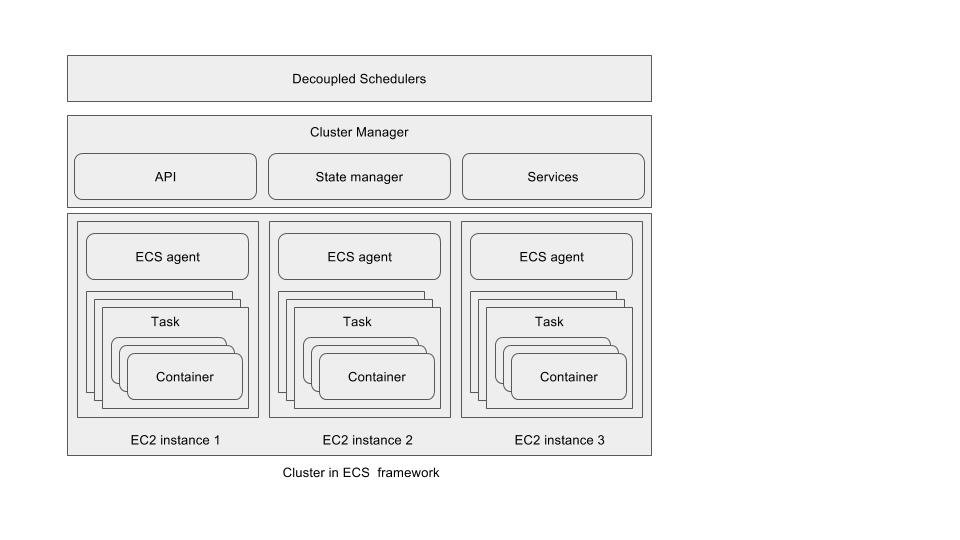
\includegraphics[scale=0.5]{./fig/ecs}
\caption{Amazon ECS Architecture}
\label{fig:ecsArch}
\end{figure*}

Amazon EC2 instances are virtual computing environment created by using the configuration template called Amazon Machine Image (AMI). AMI is preconfigured template which contains all the configuration details like services, kernel, application details etc. User can create his own image instead of using AMI. 

The instances of AMI are just like a host machine which are used to launch and deploy the applications quickly. More than one instances of a single AMI can be launched with different types. Type of the instance is used to determine the physical configuration of the host machine where the instance will be running. In case of failure of an instance, a new instance can be launched using the AMI template.

Amazon ECS has three tasks: Cluster Management Engine, state management and back-end services. Scheduler is decoupled from the cluster manager which allows the user to have their own scheduler making the scheduler as a plug-in. In ECS framework, cluster consists of a collection of EC2 instances. Each of these EC2 instances runs multiple containers. To coordinate with these EC2 instances, ECS cluster manager talks to a daemon, called ECS agent, which runs on each of these EC2 instances. ECS agents allows the ECS manager to launch, deploy and monitor the containers as per the default or the scheduler given by the user.

To coordinate with the cluster, ECS stores and maintains the cluster state information. Cluster state is stored in key/value pair. To be scalable and to avoid network or hardware failure, this key/value is distributed across the cluster. ECS uses Amazon’s core distributed system mechanism, called Paxos-based transactional journal based data store, to handle the concurrent changes in the key/value data.

ECS’s distributed cluster systems is more robust as it takes away the need to setup, run and administer the orchestration layer. 

Service discovery is not provided by ECS. You have to do the service discovery using a third party tool e.g. Zookeeper.

Following are the features of EC2 Container Service:

\begin{enumerate}
\item Compatibility with Docker containers:
ECS uses Docker containers to schedule the services and applications on the cluster of EC2 instances. Each of the EC2 instances has a Docker daemon running on them to run the container scheduled by ECS. EC2 is limited to Docker containers and not compatible with any other container platform.

\item Flexible Scheduling:
Built in scheduler of ECS will distribute the containers across the cluster to balance the requirement and availability of the resources. Decoupling of scheduler from cluster manager enables the user to integrate and use their own scheduler.

\item Task Definitions:
Task Definition is a JSON template which is used by ECS to define the tasks. Task Definition allows us to specify the requirements related to Docker image and hardware. It also allows to specify if the containers are related to each other. Multiple tasks can be launched from one task definition file. We can also have version control of the application using task definition file.

\item Scalability with high performance:
Thousands of containers can be started, stopped and managed within seconds.

\item Amazon Web Service Integration:
ECS is designed to allow the application to use other AWS features like features such as Elastic IP addresses, resource tags, IAM, CloudTrail and Virtual Private Cloud (VPC).

\end{enumerate}

In the following section, we have discussed and provided comparison of the various features of these five container orchestration tools.